\documentclass[12pt,pdf,hyperref={unicode}]{beamer}


%\documentclass[10pt]{beamer}

\usetheme[progressbar=frametitle]{metropolis}

\usepackage{booktabs}
\usepackage[scale=2]{ccicons}

\usepackage{pgfplots}
\usepgfplotslibrary{dateplot}

\usepackage{xspace}
\newcommand{\themename}{\textbf{\textsc{metropolis}}\xspace}


%\usepackage{lmodern}

% подключаем кириллицу 
\usepackage[T2A]{fontenc}
\usepackage[utf8]{inputenc}
\usepackage{listings}
%\usepackage{graphicx}
\usepackage{hyperref}

% отключить клавиши навигации
\setbeamertemplate{navigation symbols}{}

% тема оформления
\usetheme{Pittsburgh}

% цветовая схема
\usecolortheme{default}

\definecolor{light-gray}{gray}{0.90}

\title{Семинар №4}   
\subtitle{ФАКИ \the\year}
\author{Бирюков В. А.} 
\date{\today} 
% \logo{
\includegraphics[height=5mm]{images/logo.png}\vspace{-7pt}}

\begin{document}

\lstset{language=C}

% титульный слайд
\begin{frame}
\titlepage
\end{frame} 

\defverbatim[colored]\makeset{
\begin{lstlisting}[language=C++,basicstyle=\ttfamily,keywordstyle=\color{blue}]
void make_set(int X) {
  parent[X] = X;
}
\end{lstlisting}
}

\lstset{
  language=C,                % choose the language of the code
  keywordstyle=\color{blue},
  numbers=none,                   % where to put the line-numbers
  stepnumber=1,                   % the step between two line-numbers.        
  numbersep=5pt,                  % how far the line-numbers are from the code
  backgroundcolor=\color{light-gray},  % choose the background color. You must add \usepackage{color}
  showspaces=false,               % show spaces adding particular underscores
  showstringspaces=false,         % underline spaces within strings
  showtabs=false,                 % show tabs within strings adding particular underscores
  tabsize=2,                      % sets default tabsize to 2 spaces
  captionpos=b,                   % sets the caption-position to bottom
  breaklines=true,                % sets automatic line breaking
  breakatwhitespace=true,         % sets if automatic breaks should only happen at whitespace
}

\section{Массивы}

\begin{frame}[fragile]
\frametitle{Массивы} 
\begin{itemize}
\item Массив -- набор элементов, расположенных в памяти непосредственно друг за другом, доступ к которым осуществляется по индексу
\item Объявление:
\begin{lstlisting}
type arrayName [ arraySize ];
\end{lstlisting}
\item Доступ к элементу
(Нумерация в массиве начинается с 0):\\
\begin{lstlisting}
arrayName [ index ];
\end{lstlisting}
\end{itemize}
\end{frame}

\begin{frame}[fragile]
\frametitle{Массивы} 
\framesubtitle{Примеры}
Объявление:\\
\begin{lstlisting}
int array[10];
float average_temperature[12];
\end{lstlisting}
Доступ к элементу:\\
Нумерация в массиве начинается с 0\\
\begin{lstlisting}
printf("%d\n", array[9]);
average_temperature[2] = 5.2;
\end{lstlisting}
\end{frame}

\begin{frame}[fragile]
\frametitle{Массивы} 
\framesubtitle{Инициализация}
\begin{lstlisting}
int array[10];
for (int i = 0; i < 10; ++i) {
    array[i] = /* something */;
}
\end{lstlisting}
Или так:\\
\begin{lstlisting}
int array[5] = {1, 1, 2, 3, 5};
\end{lstlisting}
\end{frame}

\begin{frame}[fragile]
\frametitle{Массивы} 
\framesubtitle{Массивы в памяти}
\begin{center}
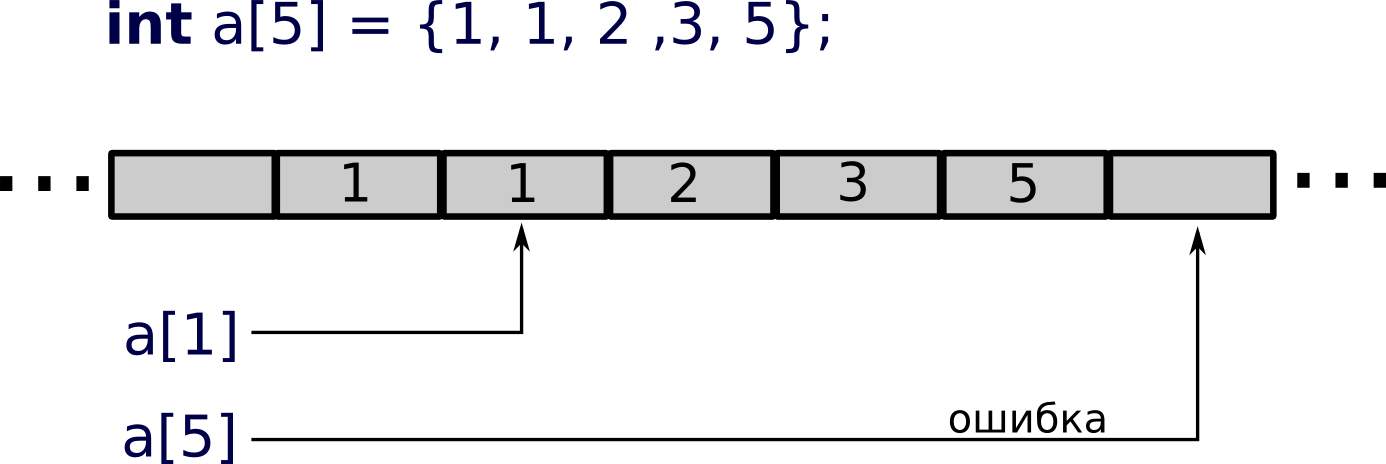
\includegraphics[width=0.95\linewidth]{images/array_in_memory.png}
\end{center}
\end{frame}


\begin{frame}[fragile]
\frametitle{Указатели и массивы} 
\framesubtitle{Указатель на элемент массива}
\begin{center}
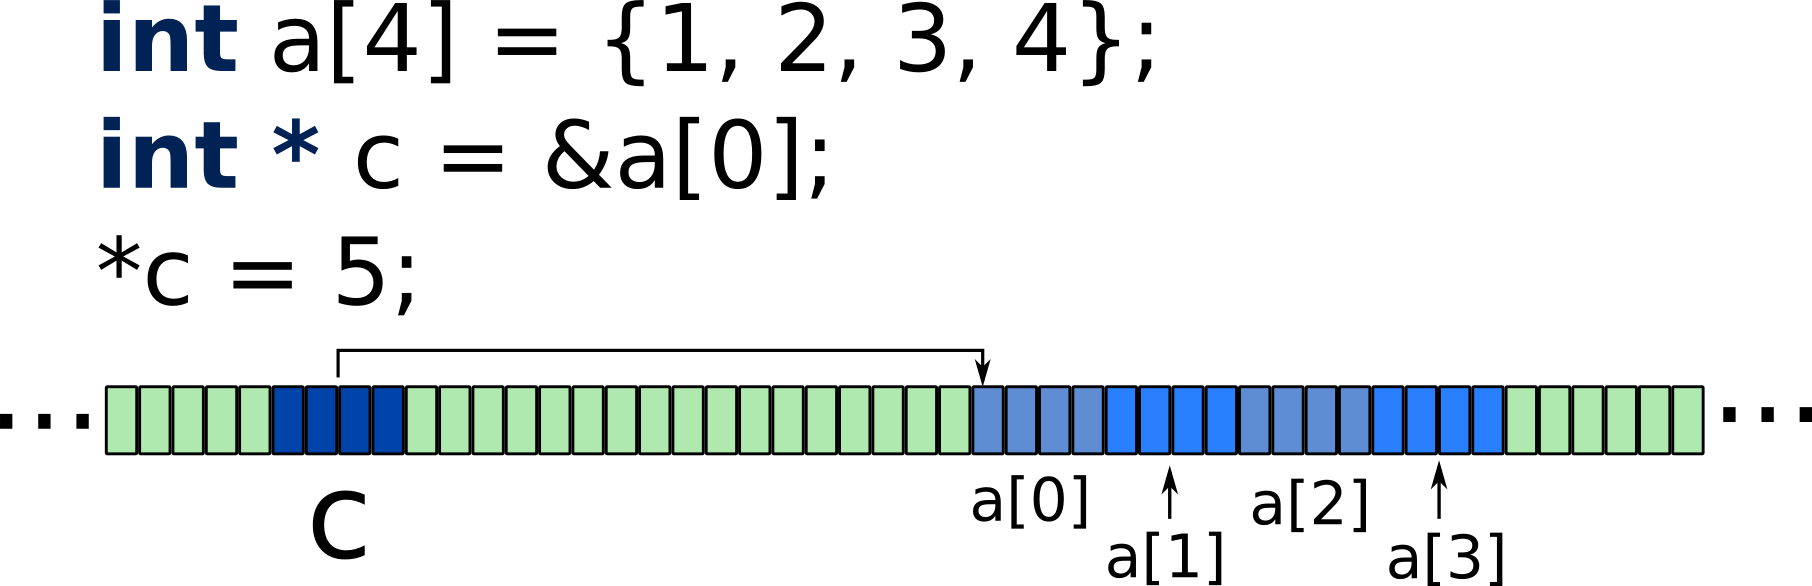
\includegraphics[width=0.95\linewidth]{images/memory_parrays_1.png}
\end{center}
\end{frame}




\section{Многомерные массивы}

\begin{frame}[fragile]
\frametitle{Многомерные массивы} 
\begin{verbatim}
type name[size1][size2]...[sizeN];
\end{verbatim}
например объявление двумерного массива:
\begin{lstlisting}[language=C++,basicstyle=\ttfamily,keywordstyle=\color{blue}]
int array[5][10];
\end{lstlisting}
задание значений:
\begin{lstlisting}[language=C++,basicstyle=\ttfamily,keywordstyle=\color{blue}, showtabs]
for (int i = 0; i < 5; ++i)
   for (int j = 0; j < 10; ++j)
       array[i][j] = something;
\end{lstlisting}
\end{frame}

\begin{frame}[fragile]
\frametitle{Двумерные массивы} 
\begin{center}
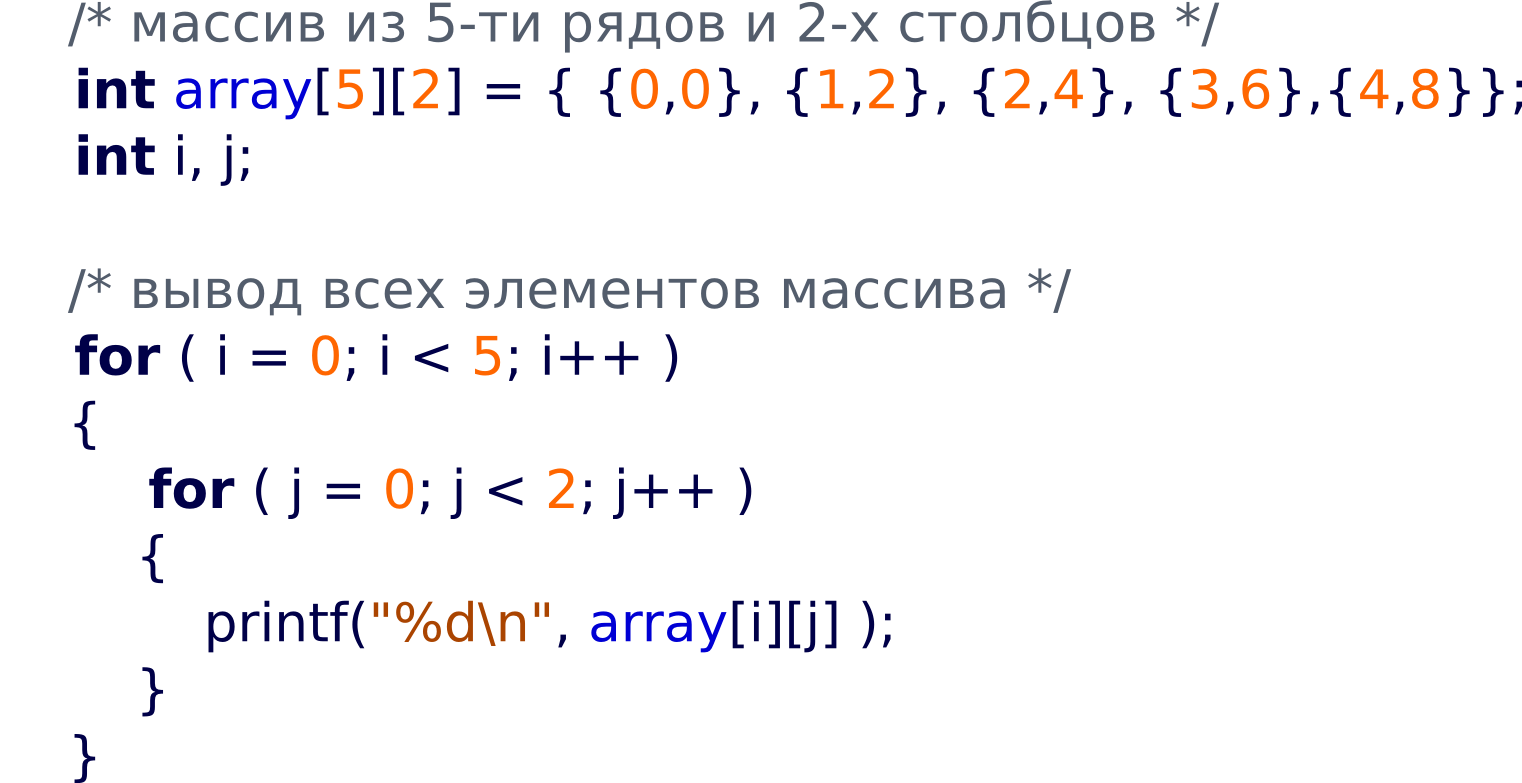
\includegraphics[scale=0.95]{images/twodim_array.png}
\end{center}
\end{frame}



\section{Введение в алгоритмы}

\begin{frame}[fragile]
\frametitle{Алгоритм} 
\begin{itemize}
\item Алгоритм -- это формально описанная вычислительная процедура, получающая исходные данные, и выдающая результат
вычислений на выход \\
(Кормен и др. "Алгоритмы: построение и анализ")
\end{itemize}
\end{frame}



\begin{frame}[fragile]
\frametitle{Задача сортировки} 
\begin{itemize}
\item Задана последовательность чисел \\
\item Нужно найти такую перестановку исходной последовательности, чтобы элементы были расположены по возрастанию  \\
\item 5 2 4 6 1 3 2 9  $\rightarrow$ 1 2 2 3 4 5 6 9
\end{itemize}
\end{frame}


\begin{frame}[fragile]
\frametitle{Простейшие сортировки} 
\begin{itemize}
\item Сортировка вставками \\
\item Сортировка выбором \\
\item Сортировка пузырьком \\
\end{itemize}
\end{frame}


\begin{frame}[fragile]
\frametitle{Анализ алгоритмов} 
\begin{itemize}
\item Обычно изучают зависимость времени работы от размера входа \\
\item Размер входа -- зависит от конкретной задачи \\
\item Для сортировки, размер входа -- это количество элементов, которые нужно отсортировать \\
\item Время работы -- число элементарных шагов, которые выполняет алгоритм
\end{itemize}
\end{frame}

\begin{frame}[fragile]
\frametitle{Пример анализа} 
\framesubtitle{Сортировка пузырьком}
\begin{lstlisting}[language=C++,basicstyle=\ttfamily,keywordstyle=\color{blue}]
for (int j = 0; j < length-1; j++)
    for (int i = 0; i < length-1; i++)
         if (a[i] > a[i+1])
             swap(&a[i], &a[i+1]);
\end{lstlisting}
функция swap(int, int) меняет значения 2-х переменных 
\begin{itemize}
\item Число операций, требуемых на один проход: $a * n$\\
\item Число проходов: $n$\\
\item Значит, время работы $\sim n^2$\\
\end{itemize}

\end{frame}




\iffalse
\begin{frame}[fragile]
\frametitle{Строки} 
\begin{itemize}
\item Строки в языке C -- на самом деле массивы из элементов типа char
\item Существенное отличие -- в конце строки должен стоять символ '\textbackslash 0'
\item Объявление:
\begin{lstlisting}
char string[10];
\end{lstlisting}
\item Доступ к элементу
(Нумерация в строке тоже начинается с 0):\\
\begin{lstlisting}
printf("%c\n", string[0]);
\end{lstlisting}
\end{itemize}
\end{frame}


\begin{frame}[fragile]
\frametitle{Строки} 
\framesubtitle{Инициализация}
\begin{lstlisting}
int string[10];
for (int i = 0; i < 10; ++i) {
    string[i] = /* something */;
}
\end{lstlisting}
Или так:\\
\begin{lstlisting}
int string[10] = {'h', 'e', 'l', 'l', 'o', '\0', 'a', 'b', 'c', 'd'};
\end{lstlisting}
Или так:\\
\begin{lstlisting}
int string[10] = "hello";
\end{lstlisting}
\end{frame}

\begin{frame}[fragile]
\frametitle{Строки} 
\framesubtitle{Строки в памяти}
\begin{center}
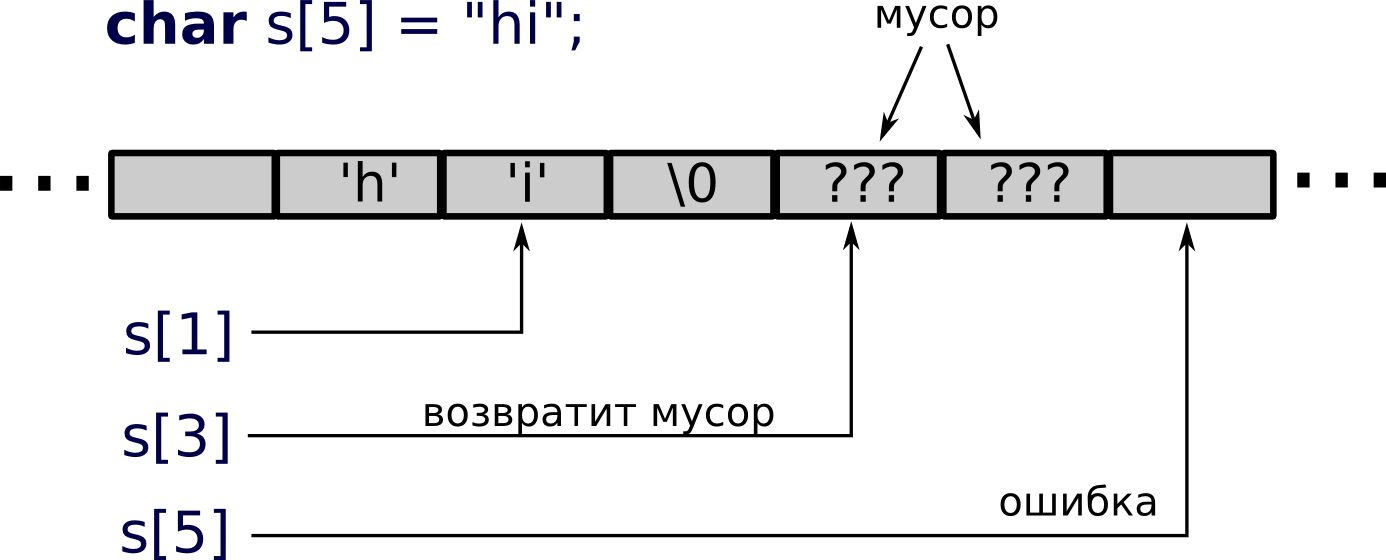
\includegraphics[width=0.95\linewidth]{images/string_in_memory.png}
\end{center}
\end{frame}

\begin{frame}[fragile]
\frametitle{Строки} 
\framesubtitle{Дополнительно}
Чтение строки:
\begin{lstlisting}
char string[10];
scanf("%10s", string);
\end{lstlisting}
Длина строки:
\begin{lstlisting}
#include <string.h>
int string[10] = "hello";
int n = strlen(string);
\end{lstlisting}
\end{frame}

\section{Примеры кода}

\begin{frame}[fragile]
\frametitle{Пример 1} 
\framesubtitle{Что делает эта программа?}
\begin{center}
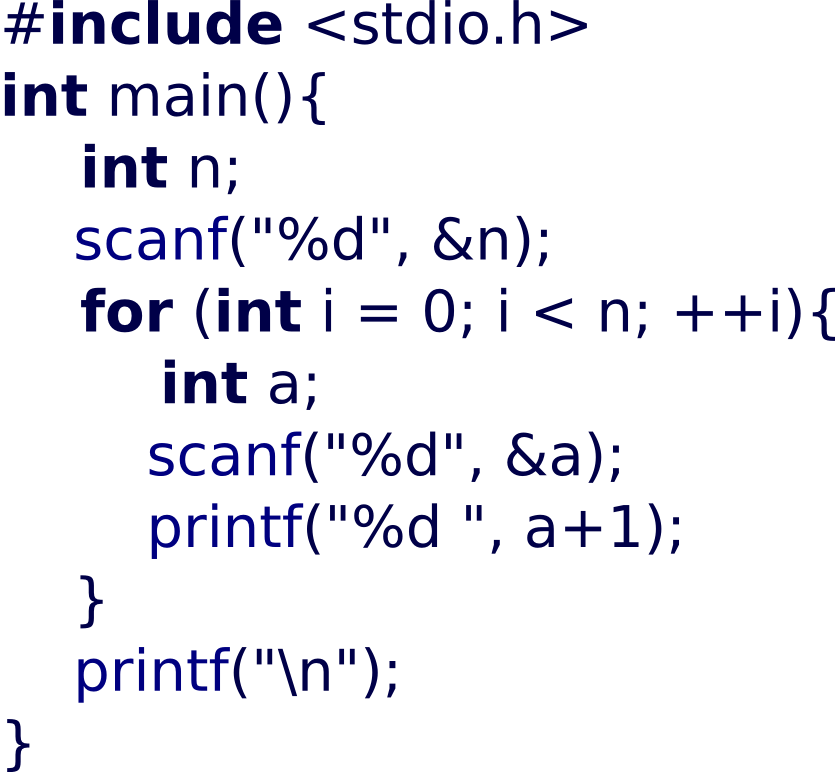
\includegraphics[width=0.62\linewidth]{images/example1.png}
\end{center}
\end{frame}

\begin{frame}[fragile]
\frametitle{Пример 2} 
\framesubtitle{Что делает эта программа?}
\begin{center}
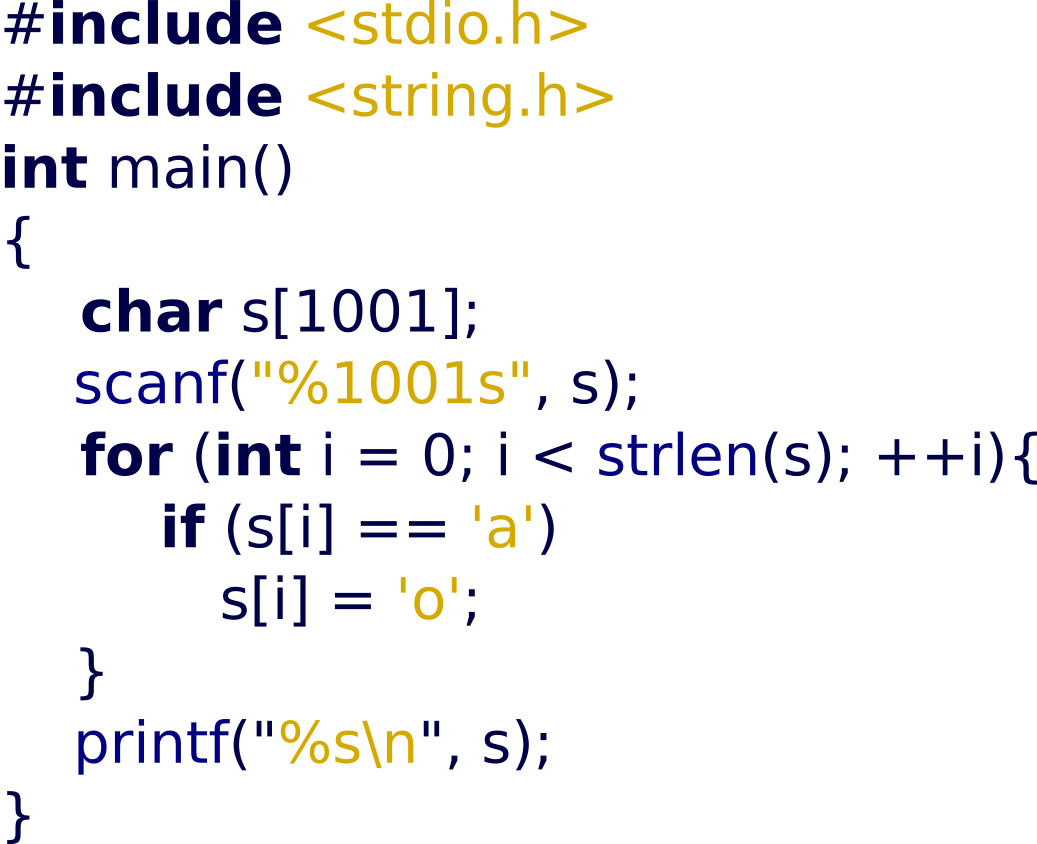
\includegraphics[width=0.62\linewidth]{images/example2.png}
\end{center}
\end{frame}

\section{Домашнее задание}

\begin{frame}
\begin{enumerate}
\item Зарегистрировать на ejudge.mipt.ru в теме "1 курс. Основные группы" ссылка "Регистрация на серию учебных контестов для первого курса"
\item Зайти на контест:\\
\url{http://kpm8.mipt.ru:8205/cgi-bin/new-client?action=207&contest_id=500102&locale_id=1}
\item Решить задачи от for\_1 до knight включительно
\end{enumerate}
\end{frame}

\fi


\end{document}
